\begin{notechapter}
\forgetcs\bA\newcommand{\bA}{\mathbf{A}}
\forgetcs\bD\newcommand{\bD}{\mathbf{D}}
\forgetcs\bL\newcommand{\bL}{\mathbf{L}}
\forgetcs\bP\newcommand{\bP}{\mathbf{P}}
\forgetcs\bI\newcommand{\bI}{\mathbf{I}}
\forgetcs\bU\newcommand{\bU}{\mathbf{U}}
\forgetcs\bM\newcommand{\bM}{\mathbf{M}}
\forgetcs\bY\newcommand{\bY}{\mathbf{Y}}
\forgetcs\bV\newcommand{\bV}{\mathbf{V}}
\forgetcs\bx\newcommand{\bx}{\mathbf{x}}
\forgetcs\by\newcommand{\by}{\mathbf{y}}
\forgetcs\bz\newcommand{\bz}{\mathbf{z}}
\forgetcs\bZ\newcommand{\bZ}{\mathbf{Z}}
\forgetcs\be\newcommand{\be}{\mathbf{e}}
\forgetcs\bv\newcommand{\bv}{\mathbf{v}}
\forgetcs\bone\newcommand{\bone}{\mathbf{1}}
\forgetcs\vol\newcommand{\vol}{\mathrm{vol}}
\forgetcs\cut\newcommand{\cut}{\mathrm{cut}}
\chapter{Graph Laplacians and Spectral Methods}\label{ch:graph-laplacians}
\chaptersubtitle{Connectivity, cuts, frequencies and embeddings from the spectrum of one matrix}

\begin{chapterintro}
The graph Laplacian $\bL = \bD - \bA$ of \cref{ch:harmonic-functions} has a spectrum that reads like a summary of
the graph. The multiplicity of its eigenvalue $0$ counts connected components; its next eigenvector
approximately splits the graph along a weak cut; and its eigenvectors, ordered by eigenvalue, are the
``frequencies'' of graph signal processing, from the smooth constant vector to signals that
change sign across every edge. This chapter proves these facts and turns them into
algorithms: spectral clustering, Laplacian eigenmaps, and smoothing by Laplacian
regularization. It follows Hamilton (\emph{Graph Representation Learning}, 2020, Chapter~2)
and von Luxburg (\emph{A Tutorial on Spectral Clustering}, 2007). You will learn
\begin{itemize}[nosep]
  \item the quadratic form $\bx^\top\bL\bx = \sum_{(i,j)\in E}(x_i - x_j)^2$ and why it measures smoothness;
  \item why the kernel of $\bL$ is spanned by the indicators of the connected components;
  \item the normalized Laplacians $\bL_{\mathrm{sym}}$ and $\bL_{\mathrm{rw}}$, and why their spectra lie in $[0, 2]$;
  \item RatioCut and its spectral relaxation, the Fiedler vector, and spectral clustering;
  \item the graph Fourier transform, and frequencies as eigenvalues of a Laplacian;
  \item Laplacian eigenmaps and the link with random-walk embeddings.
\end{itemize}
\prerequisites{\cref{ch:harmonic-functions}; the spectral theorem and the Rayleigh quotient
(\cref{ch:pca-overview}); $K$-means.}
\end{chapterintro}

\section{A running example}\label{graph-laplacians:sec:running}



Throughout this chapter we use a small graph with two communities (\cref{graph-laplacians:fig:running}):

\begin{figure}[ht]
\centering
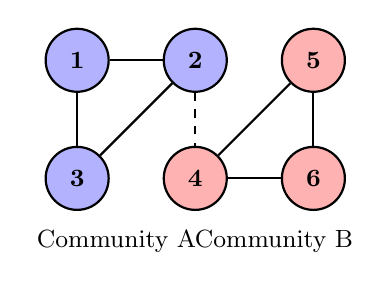
\begin{tikzpicture}[
    node distance=1.5cm,
    main/.style={circle, draw, thick, minimum size=0.8cm, font=\small\bfseries},
]
    \node[main, fill=blue!30] (1) {1};
    \node[main, fill=blue!30, right of=1] (2) {2};
    \node[main, fill=blue!30, below of=1] (3) {3};
    \node[main, fill=red!30, right of=3] (4) {4};
    \node[main, fill=red!30, right of=2] (5) {5};
    \node[main, fill=red!30, right of=4] (6) {6};

    \draw[thick] (1) -- (2);
    \draw[thick] (1) -- (3);
    \draw[thick] (2) -- (3);
    \draw[thick, dashed] (2) -- (4);
    \draw[thick] (4) -- (5);
    \draw[thick] (4) -- (6);
    \draw[thick] (5) -- (6);

    \node[below of=3, yshift=0.7cm, xshift=0.5cm, font=\small] {Community A};
    \node[below of=6, yshift=0.7cm, xshift=-0.5cm, font=\small] {Community B};
\end{tikzpicture}
\caption{The running example: two triangles joined by the bridge edge $(2, 4)$.}
\label{graph-laplacians:fig:running}
\end{figure}

The dashed edge $(2,4)$ is the ``bridge'' connecting the two communities.

%=============================================================================
\section{Matrix representations of graphs}
%=============================================================================

\subsection{Basic definitions}

Let $G = (V, E)$ be an undirected graph with $n = |V|$ nodes.

\begin{definition}[Adjacency matrix]\label{graph-laplacians:def:adjacency}
The \emph{adjacency matrix} $\bA \in \R^{n \times n}$ is defined by:
\[
\bA[i,j] = \begin{cases} 1 & \text{if } (i,j) \in E \\ 0 & \text{otherwise} \end{cases}
\]
For undirected graphs, $\bA$ is symmetric: $\bA = \bA^\top$.
\end{definition}

\begin{definition}[Degree matrix]\label{graph-laplacians:def:degree}
The \emph{degree matrix} $\bD \in \R^{n \times n}$ is a diagonal matrix with:
\[
\bD[i,i] = d_i = \sum_{j=1}^{n} \bA[i,j]
\]
where $d_i$ is the degree of node $i$.
\end{definition}

\begin{example}
For our running example:
\[
\bA = \begin{pmatrix}
0 & 1 & 1 & 0 & 0 & 0 \\
1 & 0 & 1 & 1 & 0 & 0 \\
1 & 1 & 0 & 0 & 0 & 0 \\
0 & 1 & 0 & 0 & 1 & 1 \\
0 & 0 & 0 & 1 & 0 & 1 \\
0 & 0 & 0 & 1 & 1 & 0
\end{pmatrix}, \quad
\bD = \begin{pmatrix}
2 & & & & & \\
& 3 & & & & \\
& & 2 & & & \\
& & & 3 & & \\
& & & & 2 & \\
& & & & & 2
\end{pmatrix}
\]
Node 2 (the bridge node in Community A) and node 4 (the bridge node in Community B) have degree 3.
\end{example}

%=============================================================================
\section{The graph Laplacian}
%=============================================================================

\subsection{The unnormalized (combinatorial) Laplacian}

\begin{definition}[Unnormalized Laplacian]\label{graph-laplacians:def:unnorm-laplacian}
The \emph{unnormalized Laplacian} (or combinatorial Laplacian) is:
\begin{equation}
\bL = \bD - \bA
\label{graph-laplacians:eq:laplacian}
\end{equation}
\end{definition}

\begin{example}
For our graph:
\[
\bL = \bD - \bA = \begin{pmatrix}
2 & -1 & -1 & 0 & 0 & 0 \\
-1 & 3 & -1 & -1 & 0 & 0 \\
-1 & -1 & 2 & 0 & 0 & 0 \\
0 & -1 & 0 & 3 & -1 & -1 \\
0 & 0 & 0 & -1 & 2 & -1 \\
0 & 0 & 0 & -1 & -1 & 2
\end{pmatrix}
\]

Notice the structure:
\begin{itemize}
    \item Diagonal entries: $\bL[i,i] = d_i$ (degree of node $i$).
    \item Off-diagonal: $\bL[i,j] = -1$ if $(i,j) \in E$, and $0$ otherwise.
    \item Each row sums to zero: $\sum_j \bL[i,j] = d_i - d_i = 0$.
\end{itemize}
\end{example}

\subsection{Fundamental properties of the Laplacian}

\begin{theorem}[Properties of the unnormalized Laplacian]\label{graph-laplacians:thm:laplacian-properties}
The Laplacian $\bL = \bD - \bA$ of an undirected graph satisfies:
\begin{enumerate}
    \item $\bL$ is \emph{symmetric}: $\bL = \bL^\top$.
    \item $\bL$ is \emph{positive semi-definite}: $\bx^\top \bL \bx \geq 0$ for all $\bx \in \R^n$.
    \item $\bL$ has $n$ non-negative eigenvalues: $0 = \lambda_n \leq \lambda_{n-1} \leq \cdots \leq \lambda_1$.
    \item $\bone = (1, 1, \ldots, 1)^\top$ is an eigenvector with eigenvalue $0$: $\bL \bone = \mathbf{0}$.
\end{enumerate}
\end{theorem}

\begin{proof}
\emph{(1) Symmetry}: Since $\bA$ is symmetric for undirected graphs and $\bD$ is diagonal (hence symmetric), $\bL = \bD - \bA$ is symmetric.

\emph{(2) Positive semi-definiteness}: This follows from the identity of \cref{graph-laplacians:thm:quadratic-form} below, which writes $\bx^\top\bL\bx$ as a sum of squares.

(3) Follows from (1) and (2): symmetric matrices have real eigenvalues, and positive semi-definite matrices have non-negative eigenvalues.

(4) We have $\bL \bone = (\bD - \bA)\bone = \bD\bone - \bA\bone$. Since $\bD$ is diagonal with $\bD[i,i] = d_i$, we have $(\bD\bone)[i] = d_i$. Also, $(\bA\bone)[i] = \sum_j \bA[i,j] = d_i$. Therefore $\bL\bone = \mathbf{0}$.
\end{proof}

\subsection{Graph signals}

Before diving into the key properties of the Laplacian, we need to define what a \emph{graph signal} is.

\begin{definition}[Graph signal]\label{graph-laplacians:def:graph-signal}
A \emph{graph signal} is a function $f: V \to \R$ that assigns a real value to each node. We represent it as a vector $\bx \in \R^n$ where $x_i = f(v_i)$ is the value at node $i$.
\end{definition}

\begin{example}
Concrete examples of graph signals:
\begin{itemize}
    \item \textbf{Sensor network}: Temperature measured at each sensor location.
    \item \textbf{Social network}: Age, income, or any numeric attribute of each person.
    \item \textbf{Citation network}: Number of citations for each paper.
    \item \textbf{Traffic network}: Current traffic flow at each intersection.
    \item \textbf{Binary label}: Community membership (e.g.\ $x_i = 1$ if node $i$ is in community A, $x_i = 0$ otherwise).
\end{itemize}

For our running example, the vector $\bx = (25, 30, 28, 45, 42, 48)^\top$ could represent the age of each person in the social network.
\end{example}

\begin{keyidea}
The graph structure tells us which signal values ``should be similar''. If two people are friends (connected), we might expect them to have similar ages, interests, or behaviours. The Laplacian quantifies exactly this: \emph{how much does a signal vary across edges?}
\end{keyidea}

\subsection{The Laplacian quadratic form}

The following identity is fundamental to understanding the Laplacian.

\begin{theorem}[Laplacian quadratic form]\label{graph-laplacians:thm:quadratic-form}
For any vector $\bx \in \R^n$:
\begin{equation}
\bx^\top \bL \bx = \sum_{(i,j) \in E} (x_i - x_j)^2
\label{graph-laplacians:eq:quadratic-form}
\end{equation}
\end{theorem}

\begin{proof}
We expand $\bx^\top \bL \bx = \bx^\top (\bD - \bA) \bx = \bx^\top \bD \bx - \bx^\top \bA \bx$.

\emph{First term}: Since $\bD$ is diagonal with $\bD[i,i] = d_i$:
\[
\bx^\top \bD \bx = \sum_{i=1}^{n} d_i x_i^2
\]

\emph{Second term}:
\[
\bx^\top \bA \bx = \sum_{i=1}^{n} \sum_{j=1}^{n} \bA[i,j] x_i x_j = 2 \sum_{(i,j) \in E} x_i x_j
\]
(Factor of 2 because each undirected edge is counted twice in the double sum.)

\emph{Key observation}: The degree $d_i = \sum_{j: (i,j) \in E} 1$, so:
\[
\sum_{i=1}^{n} d_i x_i^2 = \sum_{i=1}^{n} \sum_{j: (i,j) \in E} x_i^2 = \sum_{(i,j) \in E} (x_i^2 + x_j^2)
\]
(Each edge $(i,j)$ contributes $x_i^2$ to node $i$'s term and $x_j^2$ to node $j$'s term.)

\emph{Combining}:
\begin{align}
\bx^\top \bL \bx &= \sum_{(i,j) \in E} (x_i^2 + x_j^2) - 2\sum_{(i,j) \in E} x_i x_j \\
&= \sum_{(i,j) \in E} (x_i^2 - 2x_i x_j + x_j^2) \\
&= \sum_{(i,j) \in E} (x_i - x_j)^2 \qedhere
\end{align}
\end{proof}

\begin{intuition}
The quadratic form $\bx^\top \bL \bx$ measures the \emph{smoothness} of the signal $\bx$ on the graph:
\begin{itemize}
    \item If connected nodes have similar values, $(x_i - x_j)^2$ is small $\Rightarrow$ smooth signal.
    \item If connected nodes have different values, $(x_i - x_j)^2$ is large $\Rightarrow$ rough signal.
\end{itemize}

It is the discrete analogue of the Dirichlet energy $\int\norm{\nabla f}^2$ (\cref{harmonic-functions:sec:graph_laplacian}): a sum of squared \emph{first} differences
along edges, small for a function that varies slowly. The operator $\bL$ itself, whose quadratic form this
is, is the analogue of $-\Delta$.
\end{intuition}

\begin{example}
Let us compute $\bx^\top \bL \bx$ for two signals on our graph:

\emph{Smooth signal} (respects communities): $\bx_{\text{smooth}} = (1, 1, 1, 0, 0, 0)^\top$
\begin{align}
\bx_{\text{smooth}}^\top \bL \bx_{\text{smooth}} &= (1-1)^2 + (1-1)^2 + (1-1)^2 + (1-0)^2 + (0-0)^2 + (0-0)^2 + (0-0)^2 \\
&= 0 + 0 + 0 + 1 + 0 + 0 + 0 = \mathbf{1}
\end{align}
Only the bridge edge $(2,4)$ contributes.

\emph{Rough signal} (alternating): $\bx_{\text{rough}} = (1, 0, 1, 0, 1, 0)^\top$
\begin{align}
\bx_{\text{rough}}^\top \bL \bx_{\text{rough}} &= (1-0)^2 + (1-1)^2 + (0-1)^2 + (0-0)^2 + (0-1)^2 + (0-0)^2 + (1-0)^2 \\
&= 1 + 0 + 1 + 0 + 1 + 0 + 1 = \mathbf{4}
\end{align}

The smooth signal (which aligns with the community structure) has a much smaller Laplacian quadratic form than the rough signal.
\end{example}

%=============================================================================
\section{The Laplacian and graph connectivity}
%=============================================================================

One of the most elegant properties of the Laplacian is that its spectrum reveals the connectivity structure of the graph.

\begin{theorem}[Multiplicity of zero eigenvalue]\label{graph-laplacians:thm:zero-eigenvalue}
The geometric multiplicity of the eigenvalue $0$ of the Laplacian $\bL$ equals the number of connected components in the graph.
\end{theorem}

\begin{proof}
Let $\bv$ be an eigenvector of $\bL$ with eigenvalue $0$: $\bL \bv = \mathbf{0}$.

\emph{Key observation}: An eigenvector $\bv \in \R^n$ is itself a graph signal. It assigns a value $v_i$ to each node $i$. We will show that this signal must be constant within each connected component.

By the definition of eigenvalue:
\[
\bv^\top \bL \bv = \bv^\top \cdot \mathbf{0} = 0
\]

By the quadratic form identity \eqref{graph-laplacians:eq:quadratic-form}:
\[
\sum_{(i,j) \in E} (v_i - v_j)^2 = 0
\]

Since each term $(v_i - v_j)^2 \geq 0$, this sum equals zero only if \emph{every term is zero}. Therefore $v_i = v_j$ for all edges $(i,j) \in E$. In other words, the signal $\bv$ has the same value at both endpoints of every edge.

\emph{Case 1: connected graph.} If the graph is connected, then for any two nodes $u, w$, there exists a path $u = z_0, z_1, \ldots, z_k = w$. Along this path, consecutive nodes are connected by edges, so:
\[
v_u = v_{z_0} = v_{z_1} = \cdots = v_{z_k} = v_w
\]
Thus the signal $\bv$ is constant across all nodes: $\bv = c \cdot \bone$ for some constant $c$. The only eigenvector (up to scaling) is $\bone$, so the eigenvalue $0$ has multiplicity $1$.

\emph{Case 2: $K$ connected components.} If the graph has $K$ connected components $C_1, \ldots, C_K$, then by the argument above, any eigenvector for eigenvalue $0$ must be constant within each component (but can have different constants in different components).

We can construct $K$ linearly independent such eigenvectors --- the indicator signals for each component:
\[
\bv^{(k)}[i] = \begin{cases} 1 & \text{if } i \in C_k \\ 0 & \text{otherwise} \end{cases}
\]
These are orthogonal signals, each constant within its component and zero elsewhere. If we order the nodes so that each component is contiguous, the Laplacian has block diagonal structure:
\[
\bL = \begin{pmatrix} \bL_1 & & \\ & \ddots & \\ & & \bL_K \end{pmatrix}
\]
where each $\bL_k$ is the Laplacian of component $C_k$, contributing one zero eigenvalue each.
\end{proof}

\begin{remark}
The block diagonal structure only appears visually if the nodes are ordered so that each connected component is contiguous. With arbitrary node ordering, the matrix entries are scattered, but $\bL$ is still \emph{permutation-similar} to the block diagonal form: $\bL = \boldsymbol{\Pi}^\top \bL_{\text{block}} \boldsymbol{\Pi}$ for some permutation matrix $\boldsymbol{\Pi}$. Since permutation similarity preserves eigenvalues, the spectral properties (number of zero eigenvalues, etc.) do not depend on node ordering.
\end{remark}

\begin{remark}
This theorem provides an algorithmic way to count connected components: compute the eigenvalues of $\bL$ and count how many are zero (within numerical tolerance).
\end{remark}

\begin{intuition}
The proof reveals a beautiful connection: eigenvectors of $\bL$ are graph signals, and the zero-eigenvalue eigenvectors are precisely the signals that are ``perfectly smooth'' --- they do not vary across any edge. The only way to be perfectly smooth is to be constant within each connected piece of the graph.
\end{intuition}

\subsection{The kernel of the Laplacian}

From a linear algebra perspective, the eigenvalue $\lambda = 0$ means that $\ker(\bL) \neq \{\mathbf{0}\}$. For the Laplacian, this kernel has a very specific structure.

\begin{theorem}[Structure of the Laplacian kernel]\label{graph-laplacians:thm:kernel-structure}
Let $G$ have connected components $C_1, C_2, \ldots, C_K$. Then:
\begin{equation}
\ker(\bL) = \mathrm{span}\{\bone_{C_1}, \bone_{C_2}, \ldots, \bone_{C_K}\}
\end{equation}
where $\bone_{C_k} \in \R^n$ is the indicator vector for component $C_k$:
\[
\bone_{C_k}[i] = \begin{cases} 1 & \text{if } i \in C_k \\ 0 & \text{otherwise} \end{cases}
\]
In particular, $\dim(\ker(\bL)) = K$.
\end{theorem}

\begin{proof}
We established in \cref{graph-laplacians:thm:zero-eigenvalue} that any $\bv \in \ker(\bL)$ must satisfy $v_i = v_j$ for all edges $(i,j)$, which implies $\bv$ is constant on each connected component.

Any such vector can be written as $\bv = \sum_{k=1}^{K} c_k \bone_{C_k}$ where $c_k$ is the constant value on component $C_k$. Conversely, each $\bone_{C_k}$ satisfies $\bL \bone_{C_k} = \mathbf{0}$ (verify: nodes in $C_k$ have their degree cancelled by neighbour contributions, nodes outside $C_k$ contribute nothing).

Since the $\bone_{C_k}$ are linearly independent (they have disjoint support), they form a basis for $\ker(\bL)$.
\end{proof}

\begin{keyidea}
\emph{Comparing with general matrices:} For an arbitrary singular matrix $\bA$ (with $\det(\bA) = 0$), the kernel can be any subspace --- there is no particular structure. But for the Laplacian:
\begin{itemize}
    \item The kernel has dimension equal to the number of connected components.
    \item A natural basis consists of indicator vectors for each component.
    \item Every vector in $\ker(\bL)$ is ``piecewise constant'' --- constant within each component.
\end{itemize}

This is a beautiful example of how \emph{algebraic structure (the kernel) encodes topological structure (connectivity)}.
\end{keyidea}

\begin{example}
For our 6-node graph with two communities (assuming it is connected via the bridge edge), $K = 1$ and:
\[
\ker(\bL) = \mathrm{span}\{(1, 1, 1, 1, 1, 1)^\top\} = \{c \cdot \bone : c \in \R\}
\]

If we removed the bridge edge $(2,4)$, the graph would have $K = 2$ components and:
\[
\ker(\bL) = \mathrm{span}\{(1,1,1,0,0,0)^\top, (0,0,0,1,1,1)^\top\}
\]
Any vector in this kernel assigns one constant to Community A and another constant to Community B.
\end{example}

\subsection{Using eigenvectors to identify components}

The eigenvalues tell us \emph{how many} connected components exist, but can we identify \emph{which nodes belong to which component}? Yes --- the eigenvectors reveal this information.

\begin{keyidea}
For a graph with $K$ connected components, compute the $K$ eigenvectors $\bv^{(1)}, \ldots, \bv^{(K)}$ corresponding to eigenvalue $0$. Then:
\begin{center}
\emph{Two nodes $i$ and $j$ are in the same component if and only if they have the same value in every zero-eigenvalue eigenvector.}
\end{center}
\end{keyidea}

\begin{example}
Consider our 6-node running example with the bridge edge $(2,4)$ removed, creating two components: $\{1, 2, 3\}$ and $\{4, 5, 6\}$.

With our node numbering, a natural basis for $\ker(\bL)$ is:
\[
\bv^{(1)} = (1,1,1,0,0,0)^\top, \quad \bv^{(2)} = (0,0,0,1,1,1)^\top
\]

Form the matrix $\bV = [\bv^{(1)} \mid \bv^{(2)}]$ and examine each node's row:

\begin{center}
\begin{tabular}{c|cc|c}
Node & $\bv^{(1)}$ & $\bv^{(2)}$ & Row \\
\hline
1 & 1 & 0 & $(1, 0)$ \\
2 & 1 & 0 & $(1, 0)$ \\
3 & 1 & 0 & $(1, 0)$ \\
4 & 0 & 1 & $(0, 1)$ \\
5 & 0 & 1 & $(0, 1)$ \\
6 & 0 & 1 & $(0, 1)$ \\
\end{tabular}
\end{center}

Nodes 1, 2, 3 share the same row $(1, 0)$ $\Rightarrow$ same component.\\
Nodes 4, 5, 6 share the same row $(0, 1)$ $\Rightarrow$ same component.
\end{example}

\begin{remark}
The specific values in the eigenvectors depend on the node ordering and our choice of basis. For instance, if the nodes were numbered differently --- say the first component was $\{1, 3, 5\}$ and the second was $\{2, 4, 6\}$ --- we might have:
\[
\bv^{(1)} = (1,0,1,0,1,0)^\top, \quad \bv^{(2)} = (0,1,0,1,0,1)^\top
\]

Moreover, eigenvectors are only unique up to linear combinations. Any basis for $\ker(\bL)$ works. We might instead have:
\[
\tilde{\bv}^{(1)} = (3,5,3,5,3,5)^\top, \quad \tilde{\bv}^{(2)} = (2,-1,2,-1,2,-1)^\top
\]
(where $\tilde{\bv}^{(1)} = 3\bv^{(1)} + 5\bv^{(2)}$ and $\tilde{\bv}^{(2)} = 2\bv^{(1)} - \bv^{(2)}$).

The algorithm still works: nodes 1, 3, 5 all have row $(3, 2)$, and nodes 2, 4, 6 all have row $(5, -1)$. \emph{The key is that nodes in the same component have identical rows, regardless of which basis we choose.}
\end{remark}

\subsection{What about connected graphs?}

The techniques above work beautifully for disconnected graphs: zero eigenvalues and their eigenvectors directly reveal connected components. But what if the graph is connected?

\begin{intuition}
In our running example, the two communities $\{1, 2, 3\}$ and $\{4, 5, 6\}$ are connected by the bridge edge $(2, 4)$. With this edge present there is only \emph{one} zero eigenvalue (the graph is connected), and the kernel is just $\ker(\bL) = \mathrm{span}\{\bone\}$: it carries no cluster information.

Yet the community structure clearly exists. We need a different approach: instead of looking for \emph{exact} separations (disconnected components), we look for \emph{approximate} separations --- places where the graph is ``almost'' disconnected, with only a few edges crossing between groups.

This leads us to the theory of \emph{graph cuts} and \emph{spectral clustering}, which we develop after introducing normalized Laplacians.
\end{intuition}

%=============================================================================
\section{Normalized Laplacians}
%=============================================================================

The unnormalized Laplacian has a bias towards high-degree nodes. Normalized variants address this.

\subsection{The symmetric normalized Laplacian}

\begin{definition}[Symmetric normalized Laplacian]\label{graph-laplacians:def:sym-laplacian}
The \emph{symmetric normalized Laplacian} is:
\begin{equation}
\bL_{\text{sym}} = \bD^{-1/2} \bL \bD^{-1/2} = \bI - \bD^{-1/2} \bA \bD^{-1/2}
\label{graph-laplacians:eq:sym-laplacian}
\end{equation}
It requires every degree to be positive (no isolated nodes), as does $\bL_{\text{rw}}$ below.
\end{definition}

\begin{theorem}[Properties of $\bL_{\text{sym}}$]\label{graph-laplacians:thm:sym-properties}
The symmetric normalized Laplacian satisfies:
\begin{enumerate}
    \item $\bL_{\text{sym}}$ is symmetric and positive semi-definite.
    \item All eigenvalues lie in $[0, 2]$.
    \item $0$ is an eigenvalue with eigenvector $\bD^{1/2} \bone$.
    \item The quadratic form is:
    \begin{equation}
    \bx^\top \bL_{\text{sym}} \bx = \sum_{(i,j) \in E} \left( \frac{x_i}{\sqrt{d_i}} - \frac{x_j}{\sqrt{d_j}} \right)^2
    \end{equation}
\end{enumerate}
\end{theorem}

\begin{proof}
(1) $\bL_{\text{sym}} = \bD^{-1/2} \bL \bD^{-1/2}$ is symmetric since $\bL$ is symmetric and $\bD^{-1/2}$ is symmetric (diagonal with positive entries). For any $\bx$:
\[
\bx^\top \bL_{\text{sym}} \bx = \bx^\top \bD^{-1/2} \bL \bD^{-1/2} \bx = (\bD^{-1/2}\bx)^\top \bL (\bD^{-1/2}\bx) \geq 0
\]
since $\bL$ is positive semi-definite.

(2) See \cref{graph-laplacians:app:eigenvalue-bound}.

(3) $\bL_{\text{sym}} (\bD^{1/2}\bone) = \bD^{-1/2} \bL \bD^{-1/2} \bD^{1/2} \bone = \bD^{-1/2} \bL \bone = \bD^{-1/2} \cdot \mathbf{0} = \mathbf{0}$.

(4) Let $\tilde{\bx} = \bD^{-1/2}\bx$, so $\tilde{x}_i = x_i / \sqrt{d_i}$. Then:
\[
\bx^\top \bL_{\text{sym}} \bx = \tilde{\bx}^\top \bL \tilde{\bx} = \sum_{(i,j) \in E} (\tilde{x}_i - \tilde{x}_j)^2 = \sum_{(i,j) \in E} \left( \frac{x_i}{\sqrt{d_i}} - \frac{x_j}{\sqrt{d_j}} \right)^2 \qedhere
\]
\end{proof}

\begin{intuition}
The normalized quadratic form divides each node's contribution by $\sqrt{d_i}$. This means:
\begin{itemize}
    \item High-degree nodes (``celebrities'') have their influence reduced.
    \item Low-degree nodes have their influence increased.
    \item The resulting measure is more balanced across the graph.
\end{itemize}
The eigenvalue bound $[0,2]$ makes $\bL_{\text{sym}}$ easier to work with theoretically and allows comparison across graphs of different sizes.
\end{intuition}

\subsection{The random walk Laplacian}

\begin{definition}[Random walk Laplacian]\label{graph-laplacians:def:rw-laplacian}
The \emph{random walk Laplacian} is:
\begin{equation}
\bL_{\text{rw}} = \bD^{-1} \bL = \bI - \bD^{-1} \bA = \bI - \bP
\label{graph-laplacians:eq:rw-laplacian}
\end{equation}
where $\bP = \bD^{-1}\bA$ is the random walk transition matrix.
\end{definition}

\begin{theorem}[Relationship between normalized Laplacians]\label{graph-laplacians:thm:laplacian-similarity}
$\bL_{\text{rw}}$ and $\bL_{\text{sym}}$ have the same eigenvalues. If $\mathbf{v}$ is an eigenvector of $\bL_{\text{sym}}$ with eigenvalue $\lambda$, then $\bD^{-1/2}\mathbf{v}$ is an eigenvector of $\bL_{\text{rw}}$ with eigenvalue $\lambda$.
\end{theorem}

\begin{proof}
Suppose $\bL_{\text{sym}} \mathbf{v} = \lambda \mathbf{v}$. Then:
\begin{align}
(\bI - \bD^{-1/2}\bA\bD^{-1/2})\mathbf{v} &= \lambda \mathbf{v} \\
\bD^{-1/2}(\bI - \bD^{-1/2}\bA\bD^{-1/2})\mathbf{v} &= \lambda \bD^{-1/2}\mathbf{v} \\
(\bD^{-1/2} - \bD^{-1}\bA\bD^{-1/2})\mathbf{v} &= \lambda \bD^{-1/2}\mathbf{v} \\
(\bI - \bD^{-1}\bA)\bD^{-1/2}\mathbf{v} &= \lambda \bD^{-1/2}\mathbf{v} \\
\bL_{\text{rw}} (\bD^{-1/2}\mathbf{v}) &= \lambda (\bD^{-1/2}\mathbf{v}) \qedhere
\end{align}
\end{proof}

\begin{keyidea}
The connection $\bL_{\text{rw}} = \bI - \bP$ links spectral methods to random walks:
\begin{itemize}
    \item The transition matrix $\bP = \bD^{-1}\bA$ governs random walk dynamics.
    \item The eigenvalues of $\bP$ are $1 - \lambda$ where $\lambda$ are eigenvalues of $\bL_{\text{rw}}$.
    \item Methods like DeepWalk that use random walks implicitly learn spectral information.
\end{itemize}
\end{keyidea}

\subsection{Summary: three Laplacians}

\begin{center}
\begin{tabular}{lccc}
\toprule
Laplacian & Formula & Eigenvalues & Main use \\
\midrule
Unnormalized $\bL$ & $\bD - \bA$ & $[0, \infty)$ & Graph cuts, basic theory \\
Symmetric $\bL_{\text{sym}}$ & $\bI - \bD^{-1/2}\bA\bD^{-1/2}$ & $[0, 2]$ & Spectral clustering \\
Random walk $\bL_{\text{rw}}$ & $\bI - \bD^{-1}\bA$ & $[0, 2]$ & Random walks, PageRank \\
\bottomrule
\end{tabular}
\end{center}

%=============================================================================
\section{Spectral clustering}
%=============================================================================

One of the most important applications of the Laplacian is \emph{spectral clustering}: partitioning graph nodes into groups using the eigenvectors of the Laplacian.

\subsection{The problem: finding good graph partitions}

\begin{intuition}
Imagine you have a social network and want to find communities. Intuitively, a good partition should:
\begin{itemize}
    \item Have \emph{few edges between} different groups (communities are separated).
    \item Have \emph{many edges within} each group (communities are cohesive).
\end{itemize}

The challenge: this is an NP-hard combinatorial problem. We cannot try all possible partitions.

\emph{The spectral method's key insight}: We can relax the discrete problem to a continuous one, solve it using linear algebra (eigenvalues), and then round back to a discrete solution.
\end{intuition}

\subsection{Graph cuts: measuring partition quality}

\begin{definition}[Graph cut]\label{graph-laplacians:def:graph-cut}
Given a partition of nodes into disjoint sets $A$ and $\bar{A} = V \setminus A$, the \emph{cut} counts edges crossing the boundary:
\begin{equation}
\cut(A, \bar{A}) = |\{(u,v) \in E : u \in A, v \in \bar{A}\}|
\end{equation}
\end{definition}

\begin{example}
In our running example, if $A = \{1, 2, 3\}$ (Community A) and $\bar{A} = \{4, 5, 6\}$ (Community B):
\[
\cut(A, \bar{A}) = 1 \quad \text{(only the bridge edge (2,4))}
\]
This is a good cut. But if $A = \{1\}$ and $\bar{A} = \{2,3,4,5,6\}$:
\[
\cut(A, \bar{A}) = 2 \quad \text{(edges (1,2) and (1,3))}
\]
This cut is also small, but it is a terrible partition --- we just isolated one node.
\end{example}

\begin{keyidea}
Minimizing the cut alone does not work: it tends to cut off tiny pieces of the graph. We need to also encourage \emph{balanced} partitions.
\end{keyidea}

\begin{definition}[RatioCut and normalized cut]\label{graph-laplacians:def:balanced-cuts}
The \emph{RatioCut} penalizes small clusters by dividing by cluster size:
\begin{equation}
\text{RatioCut}(A, \bar{A}) = \frac{\cut(A, \bar{A})}{|A|} + \frac{\cut(A, \bar{A})}{|\bar{A}|}
\end{equation}

The \emph{Normalized Cut (NCut)} uses cluster volume (sum of degrees) instead:
\begin{equation}
\text{NCut}(A, \bar{A}) = \frac{\cut(A, \bar{A})}{\vol(A)} + \frac{\cut(A, \bar{A})}{\vol(\bar{A})}
\end{equation}
where $\vol(A) = \sum_{u \in A} d_u$.
\end{definition}

\begin{example}
Compare the two partitions from before:

\emph{Good partition} ($A = \{1,2,3\}$, $\bar{A} = \{4,5,6\}$):
\[
\text{RatioCut} = \frac{1}{3} + \frac{1}{3} = \frac{2}{3} \approx 0.67
\]

\emph{Bad partition} ($A = \{1\}$, $\bar{A} = \{2,3,4,5,6\}$):
\[
\text{RatioCut} = \frac{2}{1} + \frac{2}{5} = 2.4
\]

The RatioCut correctly identifies the community partition as better.
\end{example}

\subsection{The key connection: RatioCut and the Laplacian}

Now comes the magic: we can express RatioCut minimization as a Laplacian problem.

\begin{theorem}[RatioCut as a Laplacian problem]\label{graph-laplacians:thm:ratiocut-relaxation}
Minimizing RatioCut over all 2-partitions is equivalent to:
\begin{equation}
\min_{\mathbf{a}} \mathbf{a}^\top \bL \mathbf{a} \quad \text{subject to} \quad \mathbf{a} \perp \bone, \quad \|\mathbf{a}\|^2 = n, \quad \mathbf{a} \text{ of the two-valued form \eqref{graph-laplacians:eq:ratiocut-vector}}
\end{equation}
\end{theorem}

The proof has three parts: (1) encode a partition as a vector, (2) show this vector satisfies the constraints, (3) show $\mathbf{a}^\top \bL \mathbf{a}$ equals RatioCut (up to a constant).

\begin{proof}
\emph{Step 1: encode the partition as a vector.}
Given partition $(A, \bar{A})$, define $\mathbf{a} \in \R^n$ by:
\begin{equation}\label{graph-laplacians:eq:ratiocut-vector}
a_u = \begin{cases} +\sqrt{|\bar{A}|/|A|}  & \text{if } u \in A \\[4pt] -\sqrt{|A|/|\bar{A}|} & \text{if } u \in \bar{A} \end{cases}
\end{equation}

\emph{Why this strange formula?} The $\pm$ distinguishes the two clusters. The square root terms are chosen to make the constraints work out nicely.

\emph{Step 2: verify the constraints.}

\emph{Constraint 1: $\mathbf{a} \perp \bone$} (orthogonal to the all-ones vector)
\[
\sum_{u} a_u = |A| \cdot \sqrt{\frac{|\bar{A}|}{|A|}} - |\bar{A}| \cdot \sqrt{\frac{|A|}{|\bar{A}|}} = \sqrt{|A||\bar{A}|} - \sqrt{|A||\bar{A}|} = 0
\]

\emph{Constraint 2: $\|\mathbf{a}\|^2 = n$}
\[
\sum_{u} a_u^2 = |A| \cdot \frac{|\bar{A}|}{|A|} + |\bar{A}| \cdot \frac{|A|}{|\bar{A}|} = |\bar{A}| + |A| = n
\]

\emph{Step 3: connect to RatioCut.}
Using the Laplacian quadratic form $\mathbf{a}^\top \bL \mathbf{a} = \sum_{(u,v) \in E} (a_u - a_v)^2$:
\begin{itemize}
    \item If $u, v$ are in the \emph{same} cluster: $a_u = a_v$, so $(a_u - a_v)^2 = 0$. These edges do not contribute.
    \item If $u \in A, v \in \bar{A}$: these are cut edges, and they contribute.
\end{itemize}

For a cut edge with $u \in A, v \in \bar{A}$:
\[
(a_u - a_v)^2 = \left( \sqrt{\frac{|\bar{A}|}{|A|}} + \sqrt{\frac{|A|}{|\bar{A}|}} \right)^2 = \frac{|\bar{A}|}{|A|} + 2 + \frac{|A|}{|\bar{A}|} = \frac{(|A| + |\bar{A}|)^2}{|A| \cdot |\bar{A}|}
\]

Summing over all $\cut(A, \bar{A})$ cut edges:
\begin{align}
\mathbf{a}^\top \bL \mathbf{a} &= \cut(A, \bar{A}) \cdot \frac{n^2}{|A| \cdot |\bar{A}|} \\
&= n \cdot \cut(A, \bar{A}) \cdot \left( \frac{1}{|A|} + \frac{1}{|\bar{A}|} \right) \quad \text{(algebra)} \\
&= n \cdot \text{RatioCut}(A, \bar{A})
\end{align}

So minimizing $\mathbf{a}^\top \bL \mathbf{a}$ is equivalent to minimizing RatioCut.
\end{proof}

\subsection{The relaxation: from discrete to continuous}

\begin{keyidea}
The constraint that $\mathbf{a}$ take only the two values of \eqref{graph-laplacians:eq:ratiocut-vector} makes this problem NP-hard (we'd have to try all $2^n$ partitions).

\emph{The spectral relaxation}: Drop this constraint. Allow $\mathbf{a}$ to be any real vector satisfying $\mathbf{a} \perp \bone$ and $\|\mathbf{a}\|^2 = n$.

This relaxed problem has a beautiful closed-form solution via the Rayleigh--Ritz theorem:
\[
\min_{\substack{\mathbf{x} \perp \bone \\ \|\mathbf{x}\|^2 = n}} \mathbf{x}^\top \bL \mathbf{x} \quad \Longrightarrow \quad \mathbf{x}^* = \sqrt{n} \cdot \be_{n-1}
\]
where $\be_{n-1}$ is the \emph{Fiedler vector} --- the eigenvector for the second-smallest eigenvalue of $\bL$.
\end{keyidea}

\begin{intuition}
Why the \emph{second}-smallest eigenvector?
\begin{itemize}
    \item The smallest eigenvalue is $\lambda_n = 0$ with eigenvector $\bone$ (the constant signal).
    \item But we required $\mathbf{x} \perp \bone$, which excludes this trivial solution.
    \item So the minimum is achieved at the next eigenvector: $\be_{n-1}$ with eigenvalue $\lambda_{n-1}$.
\end{itemize}
\end{intuition}

\subsection{From eigenvector to partition}

The Fiedler vector $\be_{n-1}$ is a real-valued vector, not a partition. How do we get clusters?

\begin{keyidea}
\emph{Simple rounding}: Assign nodes to clusters based on the sign of $\be_{n-1}[u]$:
\[
u \in A \text{ if } \be_{n-1}[u] \geq 0, \qquad u \in \bar{A} \text{ if } \be_{n-1}[u] < 0
\]
\end{keyidea}

\begin{example}
For our 6-node graph, the eigenvalues of $\bL$ are $0$, $\frac{5 - \sqrt{17}}2\approx0.438$, $3$ (three times) and $\frac{5 + \sqrt{17}}2\approx4.562$, and the
Fiedler vector, normalized, is
\[
\be_5\approx(0.465,\ 0.261,\ 0.465,\ -0.261,\ -0.465,\ -0.465)^\top
\]
(up to its sign). The bridge nodes $2$ and $4$ have the smallest magnitudes: they are the least
committed to their side. The values are antisymmetric because the map $1\leftrightarrow5$, $2\leftrightarrow4$, $3\leftrightarrow6$ is a symmetry of the
graph that exchanges the two communities.

Nodes 1, 2, 3 have positive values $\Rightarrow$ Cluster A.\\
Nodes 4, 5, 6 have negative values $\Rightarrow$ Cluster B.

The spectral method perfectly recovers the two communities.
\end{example}

\subsection{The spectral clustering algorithm}

\begin{keyidea}
\emph{Spectral clustering algorithm} (for $K$ clusters):
\begin{enumerate}
    \item Compute the Laplacian $\bL$ (or $\bL_{\text{rw}}$; with $\bL_{\text{sym}}$, also normalize each row of $\bU$ to unit length before step 5).
    \item Find the $K$ eigenvectors $\be_n, \be_{n-1}, \ldots, \be_{n-K+1}$ for the $K$ smallest eigenvalues.
    \item Form matrix $\bU \in \R^{n \times K}$ with these eigenvectors as columns.
    \item Represent each node $u$ by row $\bU[u, :]$ (a $K$-dimensional vector).
    \item Run $K$-means clustering on these representations to get final clusters.
\end{enumerate}
\end{keyidea}

\begin{intuition}
Why does this work for $K > 2$ clusters?
\begin{itemize}
    \item The first eigenvector ($\lambda = 0$) is constant --- no cluster information.
    \item The second eigenvector solves the relaxed RatioCut problem, and its signs give an approximate split into 2 parts.
    \item The third eigenvector provides the next best ``direction'' of separation.
    \item Together, $K$ eigenvectors embed nodes so that cluster structure becomes apparent in Euclidean space.
\end{itemize}

Nodes in the same cluster end up with similar eigenvector coordinates, so $K$-means can find them.
\end{intuition}

\subsection{The big picture: from disconnected to connected}

Now that we have developed the theory of spectral clustering, let us step back and see how everything fits together. The key insight is that \emph{disconnected components} and \emph{soft clusters} are two ends of a spectrum.

\begin{keyidea}
The eigenvalues of the Laplacian measure how ``separable'' the graph is:

\begin{center}
\begin{tabular}{cl}
\toprule
Eigenvalue & What it reveals \\
\midrule
$\lambda_n = 0$ & Graph is connected (multiplicity $>1$ means disconnected) \\
$\lambda_{n-1}$ small & Graph is ``almost'' disconnected --- good 2-way cut exists \\
$\lambda_{n-2}$ small & Good 3-way partition exists \\
\vdots & \vdots \\
\bottomrule
\end{tabular}
\end{center}

\emph{Small eigenvalues = weak connections between parts of the graph.}
\end{keyidea}

\begin{intuition}
Consider what happens as we vary the bridge edge in our running example:

\emph{Bridge removed} (disconnected): $\lambda_6 = \lambda_5 = 0$. The two zero-eigenvalue eigenvectors are exactly constant within each component:
\[
\bv^{(1)} = (1,1,1,0,0,0)^\top, \quad \bv^{(2)} = (0,0,0,1,1,1)^\top
\]
Cluster identification is trivial: nodes with the same values are in the same component.

\emph{Bridge present} (connected): Now $\lambda_6 = 0$ and $\lambda_5 = (5 - \sqrt{17})/2\approx0.438 > 0$ (small, because only one edge connects the communities). The Fiedler vector is \emph{almost} constant within each community:
\[
\be_5 \approx (0.465, 0.261, 0.465, -0.261, -0.465, -0.465)^\top
\]
The values are not exactly equal within each community, but they are close --- and crucially, they have opposite signs across the cut. Thresholding at zero recovers the communities.

\emph{Many bridges added}: As we add more edges between communities, $\lambda_5$ grows larger. The Fiedler vector becomes less ``clean'' --- the communities are harder to separate because they are more interconnected.
\end{intuition}

\begin{definition}[Algebraic connectivity]\label{graph-laplacians:def:algebraic-connectivity}
The second-smallest eigenvalue $\lambda_{n-1}$ of the Laplacian is called the \emph{algebraic connectivity} or \emph{Fiedler value}. It quantifies how strongly connected the graph is:
\begin{itemize}
    \item $\lambda_{n-1} = 0$: Graph is disconnected.
    \item $\lambda_{n-1}$ small: Graph has a bottleneck (sparse cut).
    \item $\lambda_{n-1}$ large: Graph is well-connected (no easy cuts).
\end{itemize}
\end{definition}

\begin{remark}
This explains why spectral clustering works: we are looking for structure that is ``almost disconnected''. The smallest non-zero eigenvalues correspond to the weakest connections in the graph, and their eigenvectors reveal where to cut. Spectral clustering is really just a continuous relaxation of the problem of finding disconnected components.
\end{remark}

%=============================================================================
\section{Graph signal processing perspective}
%=============================================================================

We introduced graph signals in \cref{graph-laplacians:def:graph-signal} as vectors $\bx \in \R^n$ assigning values to nodes. Now we develop a more sophisticated view: we can analyse signals in terms of their ``frequency content'' on the graph, analogous to Fourier analysis for time-domain signals.

\subsection{The graph Fourier transform}

\begin{definition}[Graph Fourier transform]\label{graph-laplacians:def:gft}
The eigenvectors of $\bL$ form an orthonormal basis $\{\be_1, \ldots, \be_n\}$ for $\R^n$. Any graph signal $\bx$ can be decomposed in this basis. The \emph{Graph Fourier Transform (GFT)} gives the coefficients:
\begin{equation}
\hat{x}_k = \langle \bx, \be_k \rangle = \be_k^\top \bx
\end{equation}
The inverse transform reconstructs the signal: $\bx = \sum_{k=1}^{n} \hat{x}_k \be_k$.
\end{definition}

\begin{intuition}
The eigenvalues $\lambda_k$ act like ``frequencies'':
\begin{itemize}
    \item \textbf{Small $\lambda_k$}: The eigenvector $\be_k$ is a smooth signal (low frequency). Connected nodes have similar values.
    \item \textbf{Large $\lambda_k$}: The eigenvector $\be_k$ oscillates rapidly across edges (high frequency). Connected nodes have different values.
\end{itemize}
This follows directly from the quadratic form: $\be_k^\top \bL \be_k = \lambda_k$ measures how much $\be_k$ varies across edges.

The eigenvector $\be_n$ with $\lambda_n = 0$ is the constant signal $\bone$ --- the smoothest possible signal with zero variation. The eigenvector $\be_1$ with the largest eigenvalue is the ``most oscillatory'' signal on the graph.
\end{intuition}

\subsection{Frequencies as eigenvalues of a Laplacian}\label{graph-laplacians:sec:frequencies}

The name ``Fourier transform'' is more than an analogy. The complex exponentials $e^{i\omega t}$ of classical
Fourier analysis are eigenfunctions of the second derivative, $\frac{d^2}{dt^2}e^{i\omega t} = -\omega^2e^{i\omega t}$: the classical Fourier transform is
the spectral decomposition of the one-dimensional Laplacian, and the frequency $\omega$ is read from the
eigenvalue $-\omega^2$. On the real line or on a regular grid, translation invariance makes these eigenfunctions
the same for every problem, so the Laplacian that generates them is rarely mentioned; on a
cycle graph, the eigenvectors of $\bL$ are exactly the discrete Fourier basis (\cref{ch:dft-to-gnn}). A general graph has no
translations, and its ``sines and cosines'' must be computed by diagonalizing its own $\bL$. In both
cases, frequency is a rate of variation, measured by the eigenvalue: $\be_k^\top\bL\be_k = \lambda_k$ is the Dirichlet energy of the
$k$-th basis signal.

\subsection{Smoothness and regularization}

\begin{keyidea}
In many applications, we want to find a smooth signal on the graph. This leads to the regularized optimization:
\begin{equation}
\min_{\bx} \| \bx - \by \|^2 + \alpha \cdot \bx^\top \bL \bx
\end{equation}
where $\by$ is observed data and $\alpha > 0$ controls smoothness. The first term fits the data; the second penalizes non-smooth signals.
Setting the gradient $2(\bx - \by) + 2\alpha\bL\bx$ to zero gives the unique solution $\bx^* = (\bI + \alpha\bL)^{-1}\by$, and in the Fourier
basis $\hat x^*_k = \hat y_k/(1 + \alpha\lambda_k)$: a low-pass filter that shrinks each frequency by $1/(1 + \alpha\lambda_k)$.

This framework underlies:
\begin{itemize}
    \item Label propagation for semi-supervised learning.
    \item Graph-based image denoising.
    \item Network regularization in machine learning.
\end{itemize}
\end{keyidea}

%=============================================================================
\section{Connection to node embeddings}
%=============================================================================

\subsection{Laplacian eigenmaps}

\begin{definition}[Laplacian eigenmaps]\label{graph-laplacians:def:laplacian-eigenmaps}
The \emph{Laplacian Eigenmaps} algorithm (Belkin and Niyogi, \emph{Laplacian Eigenmaps for
Dimensionality Reduction and Data Representation}, 2003) solves the generalized eigenproblem
$\bL\bv = \lambda\bD\bv$, equivalently $\bL_{\text{rw}}\bv = \lambda\bv$, and embeds node $u$ as
\begin{equation}
\by_u = (\bv_2[u], \bv_3[u], \ldots, \bv_{d+1}[u])^\top,
\end{equation}
where $\bv_1 = \bone$ (eigenvalue $0$), $\bv_2, \bv_3,\dots$ are the generalized eigenvectors for the next smallest eigenvalues. It is
the spectral clustering representation built from $\bL_{\text{rw}}$, without the $K$-means step.
\end{definition}

\begin{theorem}[Laplacian eigenmaps optimality]\label{graph-laplacians:thm:eigenmaps-optimal}
Laplacian Eigenmaps solves:
\begin{equation}
\min_{\bY \in \R^{n \times d}} \sum_{(i,j) \in E} \| \by_i - \by_j \|^2 = \tr(\bY^\top\bL\bY) \quad \text{subject to} \quad \bY^\top \bD \bY = \bI,\quad\bY^\top\bD\bone = \mathbf 0,
\end{equation}
where $\by_i^\top$ is row $i$ of $\bY$.
\end{theorem}

\begin{proof}
Substitute $\bZ = \bD^{1/2}\bY$: the problem becomes $\min\tr(\bZ^\top\bL_{\text{sym}}\bZ)$ subject to $\bZ^\top\bZ = \bI$ and $\bZ^\top\bD^{1/2}\bone = \mathbf 0$. The
minimum of $\tr(\bZ^\top\bM\bZ)$ over matrices with $d$ orthonormal columns orthogonal to the eigenvector $\bD^{1/2}\bone$ of
$\bM = \bL_{\text{sym}}$ for the eigenvalue $0$ is the sum of the next $d$ eigenvalues, attained by the corresponding
eigenvectors (Ky Fan's theorem, the multi-vector form of Rayleigh--Ritz). By
\cref{graph-laplacians:thm:laplacian-similarity}, $\bY = \bD^{-1/2}\bZ$ then consists of eigenvectors of $\bL_{\text{rw}}$.
\end{proof}

\begin{intuition}
The objective encourages connected nodes to have nearby embeddings. The constraint prevents the trivial solution where all embeddings collapse to a single point.
\end{intuition}

\subsection{Connection to random walk methods}

Methods like DeepWalk and node2vec use random walks to generate node embeddings. These are deeply connected to the Laplacian:

\begin{keyidea}
With window size $T$ and $b$ negative samples, DeepWalk with negative sampling implicitly factorizes
(Qiu et al., \emph{Network Embedding as Matrix Factorization}, 2018)
\begin{equation}
\bM = \log\Bigl(\frac{\vol(G)}{bT}\Bigl(\sum_{t=1}^{T}\bP^t\Bigr)\bD^{-1}\Bigr),
\end{equation}
the logarithm being taken entrywise, where $\bP = \bD^{-1}\bA = \bI - \bL_{\text{rw}}$ is the random walk transition matrix and
$\vol(G) = \sum_id_i$. The sum $\sum_t\bP^t$ is a polynomial in $\bL_{\text{rw}}$, with the same eigenvectors; the entrywise logarithm
breaks this, so random-walk embeddings are close relatives of Laplacian eigenmaps, not the same
method (\cref{ch:shallow-embeddings}).
\end{keyidea}

\begin{chaptersummary}
\begin{itemize}
  \item $\bL = \bD - \bA$ is symmetric positive semi-definite, $\bL\bone = \mathbf 0$, and $\bx^\top\bL\bx = \sum_{(i,j)\in E}(x_i - x_j)^2$ measures the variation of a
        signal across edges.
  \item $\ker\bL$ is spanned by the indicators of the connected components: the multiplicity of $0$ counts
        components.
  \item $\bL_{\text{sym}} = \bI - \bD^{-1/2}\bA\bD^{-1/2}$ and $\bL_{\text{rw}} = \bI - \bD^{-1}\bA$ are similar, with eigenvalues in $[0, 2]$; $\bL_{\text{rw}}$ is tied to random walks.
  \item RatioCut equals $\frac1n\mathbf a^\top\bL\mathbf a$ for a two-valued vector; relaxing the two values gives the Fiedler vector, the
        eigenvector of the second-smallest eigenvalue, and spectral clustering runs $K$-means on the
        $K$ eigenvectors with the smallest eigenvalues.
  \item The eigenvectors of $\bL$ are the graph Fourier basis, with eigenvalues as frequencies; Laplacian
        regularization $(\bI + \alpha\bL)^{-1}\by$ is a low-pass filter.
  \item Laplacian eigenmaps embed nodes with generalized eigenvectors $\bL\bv = \lambda\bD\bv$; random-walk embeddings factorize a
        nonlinear function of powers of $\bP = \bI - \bL_{\text{rw}}$.
\end{itemize}
\end{chaptersummary}

\chapterappendix
\section{Additional proofs}
%=============================================================================

\subsection{Eigenvalue bound for $\bL_{\text{sym}}$}
\label{graph-laplacians:app:eigenvalue-bound}

\begin{proposition}[Eigenvalue bound]\label{graph-laplacians:prop:eigenvalue-bound}
All eigenvalues of $\bL_{\text{sym}}$ lie in $[0, 2]$.
\end{proposition}

\begin{proof}
The proof has two parts: (1) bound the quadratic form, then (2) connect to eigenvalues.

\emph{Part 1: bounding the quadratic form.} We already know $\bx^\top\bL_{\text{sym}}\bx\geq0$. For the upper bound, use the quadratic form
of \cref{graph-laplacians:thm:sym-properties} and $(a - b)^2\leq2a^2 + 2b^2$:
\[
\bx^\top\bL_{\text{sym}}\bx = \sum_{(i,j)\in E}\Bigl(\frac{x_i}{\sqrt{d_i}} - \frac{x_j}{\sqrt{d_j}}\Bigr)^2
\leq 2\sum_{(i,j)\in E}\Bigl(\frac{x_i^2}{d_i} + \frac{x_j^2}{d_j}\Bigr) = 2\sum_{i=1}^n x_i^2,
\]
because node $i$ is an endpoint of exactly $d_i$ edges, each contributing $x_i^2/d_i$. Hence $0\leq\bx^\top\bL_{\text{sym}}\bx\leq2$ for every
unit vector $\bx$. (Equality in the upper bound needs $x_i/\sqrt{d_i} = -x_j/\sqrt{d_j}$ on every edge: the eigenvalue $2$ occurs exactly
for bipartite components.)

\emph{Part 2: from quadratic form bounds to eigenvalue bounds.}
For any symmetric matrix $\bM$, the Rayleigh--Ritz theorem (\cref{graph-laplacians:thm:rayleigh-ritz}) states:
\[
\lambda_{\min}(\bM) = \min_{\|\bx\| = 1} \bx^\top \bM \bx, \qquad \lambda_{\max}(\bM) = \max_{\|\bx\| = 1} \bx^\top \bM \bx
\]

Since we proved $0 \leq \bx^\top \bL_{\text{sym}} \bx \leq 2$ for all unit vectors $\bx$, it follows that:
\[
\lambda_{\min}(\bL_{\text{sym}}) \geq 0 \quad \text{and} \quad \lambda_{\max}(\bL_{\text{sym}}) \leq 2
\]

Therefore all eigenvalues lie in $[0, 2]$.
\end{proof}

\subsection{Rayleigh--Ritz theorem}

\begin{theorem}[Rayleigh--Ritz]\label{graph-laplacians:thm:rayleigh-ritz}
Let $\bM$ be a symmetric matrix with eigenvalues $\lambda_1 \geq \lambda_2 \geq \cdots \geq \lambda_n$ and corresponding orthonormal eigenvectors $\be_1, \ldots, \be_n$. Then:
\begin{equation}
\min_{\bx \neq \mathbf{0}} \frac{\bx^\top \bM \bx}{\bx^\top \bx} = \lambda_n
\end{equation}
with minimum achieved at $\bx = \be_n$.

More generally:
\begin{equation}
\min_{\substack{\bx \neq \mathbf{0} \\ \bx \perp \be_n, \ldots, \be_{n-k+2}}} \frac{\bx^\top \bM \bx}{\bx^\top \bx} = \lambda_{n-k+1}
\end{equation}
\end{theorem}

\section*{Further reading}
\addcontentsline{toc}{section}{Further reading}
Hamilton, \emph{Graph Representation Learning}, 2020, Chapters 1--2; von Luxburg, \emph{A Tutorial on
Spectral Clustering}, 2007; Chung, \emph{Spectral Graph Theory}, 1997; Ortega et al., \emph{Graph Signal
Processing: Overview, Challenges, and Applications}, 2018.

\section*{Exercises}
\addcontentsline{toc}{section}{Exercises}

\begin{exercise}\label{graph-laplacians:exr:1}
Compute $\bL$ and its eigenvalues for the path with $3$ nodes and for the star with $4$ nodes (one centre
joined to $3$ leaves). How many times does each eigenvalue occur?
\solutionlink{graph-laplacians:exr:1}
\end{exercise}

\begin{exercise}\label{graph-laplacians:exr:2}
In the running example, compute RatioCut and NCut for the partitions $\{1, 2, 3\}\mid\{4, 5, 6\}$ and $\{1, 3\}\mid\{2, 4, 5, 6\}$.
\solutionlink{graph-laplacians:exr:2}
\end{exercise}

\begin{exercise}\label{graph-laplacians:exr:3}
Show that $2$ is an eigenvalue of $\bL_{\text{sym}}$ for a connected graph if and only if the graph is bipartite.
\hint{Use the equality case of the bound in the appendix.}
\solutionlink{graph-laplacians:exr:3}
\end{exercise}

\begin{exercise}\label{graph-laplacians:exr:4}
For the cycle with $n$ nodes, show that $\bv_k = (\cos(2\pi kj/n))_{j=0}^{n-1}$ is an eigenvector of $\bL$, with eigenvalue $2 - 2\cos(2\pi k/n)$.
\solutionlink{graph-laplacians:exr:4}
\end{exercise}

\begin{exercise}\label{graph-laplacians:exr:5}
Smooth the signal $\by = (1, 1, 0, 1, 0, 0)$ on the running example with $\alpha = 1$, $\bx^* = (\bI + \bL)^{-1}\by$. Compare the distances of $\by$ and $\bx^*$ to
$\mathbf t = (1, 1, 1, 0, 0, 0)$, and say whether thresholding $\bx^*$ at $\frac12$ recovers $\mathbf t$. Explain with the Fourier coefficients of $\by$.
\solutionlink{graph-laplacians:exr:5}
\end{exercise}
\end{notechapter}
